
\documentclass[border=8pt, multi, tikz]{standalone} 
\usepackage{import}
\subimport{../layers/}{init}
\usetikzlibrary{positioning}
\usetikzlibrary{3d} %for including external image 
\usepackage{amsbsy}
\usepackage{amsmath}

\def\ConvColor{rgb:yellow,5;red,2.5;white,5}
\def\ConvReluColor{rgb:yellow,5;red,5;white,5}
\def\PoolColor{rgb:red,1;black,0.3}
\def\UnpoolColor{rgb:magenta,5;black,20}
\def\ResBlocksColor{rgb:blue,5;black,30}
\def\StrideOneColor{rgb:blue,5;red,2.5;white,5}
\def\StrideTwoColor{rgb:red,1;black,0.3}
\def\TransConvColor{rgb:blue,2;green,1;black,0.3}
\def\AffineColor{rgb:yellow,5;red,2.5;white,5}
\def\FcColor{rgb:blue,5;red,2.5;white,5}
\def\FcReluColor{rgb:blue,5;red,5;white,4}
\def\SoftmaxColor{rgb:magenta,5;black,7}   
\def\SumColor{rgb:blue,5;green,15}
\def\ConcatColor{rgb:blue,5;red,2.5;white,5}

\newcommand{\copymidarrow}{\tikz \draw[-Stealth,line width=0.8mm,draw={rgb:blue,4;red,1;green,1;black,3}] (-0.3,0) -- ++(0.3,0);}

\begin{document}
\begin{tikzpicture}
\tikzstyle{connection}=[ultra thick,every node/.style={sloped,allow upside down},draw=\edgecolor,opacity=0.7]
\tikzstyle{copyconnection}=[ultra thick,every node/.style={sloped,allow upside down},draw={rgb:blue,4;red,1;green,1;black,3},opacity=0.7]

\pic[shift={ (-3, 0, 0) }] at (0,0,0) 
    {RightBandedBox={
        name=any,
        caption= ,
        xlabel={{1, }},
        zlabel=256,
        fill=\ConvColor,
        bandfill=\ConvReluColor,
        height=32,
        width=0.01,
        depth=32,
        opacity = 0.6,
        bandopacity = 0.6
        }
    };

\node[canvas is zy plane at x=0] (input) at (-3, 0, 0) {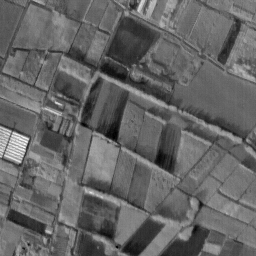
\includegraphics[width=6.4cm,height=6.4cm]{../pan_real.png}};
\coordinate (input-east) at (-3, 0, 0);

\pic[shift={(3.5,0,0)}] at (input-east) 
    {Box={
        name=cnr_b0_conv,
        caption= ,
        xlabel={{64, }},
        zlabel=,
        fill = \StrideOneColor,
        height=32,
        width=1.7777777777777777,
        depth=32,
        xlabeloc=0.5,
        }
    };

\draw [connection]  (input-east)    -- node {\midarrow}  (cnr_b0_conv-west);

\pic[shift={ (0,0,0) }] at (cnr_b0_conv-east) 
    {RightBandedBox={
        name=cnr_b0,
        caption= ,
        xlabel={{, }},
        zlabel=256,
        fill=\ConvColor,
        bandfill=\ConvReluColor,
        height=32,
        width=0.5,
        depth=32,
        opacity = 0.6,
        bandopacity = 0.6
        }
    };

\pic[shift={(3,0,0)}] at (cnr_b0-east) 
    {Box={
        name=cnr_b1_conv,
        caption= ,
        xlabel={{64, }},
        zlabel=256,
        fill = \StrideTwoColor,
        height=32,
        width=1.7777777777777777,
        depth=32,
        xlabeloc=0.5,
        }
    };

\draw [connection]  (cnr_b0-east)    -- node {\midarrow}  (cnr_b1_conv-west);

\pic[shift={ (0,0,0) }] at (cnr_b1_conv-east) 
    {RightBandedBox={
        name=cnr_b1,
        caption= ,
        xlabel={{, }},
        zlabel=,
        fill=\ConvColor,
        bandfill=\ConvReluColor,
        height=16,
        width=0.5,
        depth=16,
        opacity = 0.6,
        bandopacity = 0.6
        }
    };

\pic[shift={(2.5,0,0)}] at (cnr_b1-east) 
    {Box={
        name=cnr_b2_conv,
        caption= ,
        xlabel={{128, }},
        zlabel=128,
        fill = \StrideTwoColor,
        height=16.0,
        width=3.5555555555555554,
        depth=16.0,
        xlabeloc=0.5,
        }
    };

\draw [connection]  (cnr_b1-east)    -- node {\midarrow}  (cnr_b2_conv-west);

\pic[shift={ (0,0,0) }] at (cnr_b2_conv-east) 
    {RightBandedBox={
        name=cnr_b2,
        caption= ,
        xlabel={{, }},
        zlabel=,
        fill=\ConvColor,
        bandfill=\ConvReluColor,
        height=8,
        width=0.5,
        depth=8,
        opacity = 0.6,
        bandopacity = 0.6
        }
    };
\node[rectangle,
        draw,
dashed,
        ultra thick,
        minimum width = 9.5cm,
        minimum height = 11cm,        
        label=below:\Huge {Encoder}](r) at([xshift=-1.85em, yshift=0em]cnr_b1-anchor) {\Huge };
    
\pic[shift={(2,0,0)}] at (cnr_b2-east) 
    {Box={
        name=res_blocks_0,
        caption= ,
        xlabel={{256, }},
        zlabel=64,
        fill = \ResBlocksColor,
        height=8.0,
        width=7.111111111111111,
        depth=8.0,
        xlabeloc=0.5,
        }
    };

\draw [connection]  (cnr_b2-east)    -- node {\midarrow}  (res_blocks_0-west);
\node[rectangle,
        dashed,
        ultra thick,
        minimum width = 3cm,
        minimum height = 4cm,        
        label=below:\Huge {$\times 6$}](hdots) at([xshift=9em, yshift=0em]res_blocks_0-east) {\Huge $\pmb{\cdots}$};
    
\draw [connection]  (res_blocks_0-east)    -- node {\midarrow}  (hdots.west);

\pic[shift={(1.5,0,0)}] at (hdots.east) 
    {Box={
        name=res_blocks_5,
        caption= ,
        xlabel={{256, }},
        zlabel=64,
        fill = \ResBlocksColor,
        height=8.0,
        width=7.111111111111111,
        depth=8.0,
        xlabeloc=0.5,
        }
    };

\draw [connection]  (hdots.east)    -- node {\midarrow}  (res_blocks_5-west);
\node[rectangle,
        draw,
dashed,
        ultra thick,
        minimum width = 10.5cm,
        minimum height = 6cm,        
        label=below:\Huge {Bottleneck}](bottleneck) at([xshift=-0.25em, yshift=0em]hdots.center) {\Huge };
    
\pic[shift={(2,0,0)}] at (res_blocks_5-east) 
    {Box={
        name=cnr_b4_conv,
        caption= ,
        xlabel={{256, }},
        zlabel=,
        fill = \TransConvColor,
        height=8.0,
        width=7.111111111111111,
        depth=8.0,
        xlabeloc=0.3,
        }
    };

\draw [connection]  (res_blocks_5-east)    -- node {\midarrow}  (cnr_b4_conv-west);

\pic[shift={ (0,0,0) }] at (cnr_b4_conv-east) 
    {RightBandedBox={
        name=cnr_b4,
        caption= ,
        xlabel={{, }},
        zlabel=,
        fill=\ConvColor,
        bandfill=\ConvReluColor,
        height=16,
        width=0.5,
        depth=16,
        opacity = 0.6,
        bandopacity = 0.6
        }
    };

\pic[shift={(2,0,0)}] at (cnr_b4-east) 
    {Box={
        name=cnr_b5_conv,
        caption= ,
        xlabel={{128, }},
        zlabel=,
        fill = \TransConvColor,
        height=16.0,
        width=3.5555555555555554,
        depth=16.0,
        xlabeloc=-0.75,
        }
    };

\draw [connection]  (cnr_b4-east)    -- node {\midarrow}  (cnr_b5_conv-west);

\pic[shift={ (0,0,0) }] at (cnr_b5_conv-east) 
    {RightBandedBox={
        name=cnr_b5,
        caption= ,
        xlabel={{, }},
        zlabel=,
        fill=\ConvColor,
        bandfill=\ConvReluColor,
        height=32,
        width=0.5,
        depth=32,
        opacity = 0.6,
        bandopacity = 0.6
        }
    };

\pic[shift={(3,0,0)}] at (cnr_b5-east) 
    {Box={
        name=cnr_b6_conv,
        caption= ,
        xlabel={{64, }},
        zlabel=,
        fill = \StrideOneColor,
        height=32,
        width=1.7777777777777777,
        depth=32,
        xlabeloc=0.5,
        }
    };

\draw [connection]  (cnr_b5-east)    -- node {\midarrow}  (cnr_b6_conv-west);

\pic[shift={ (0,0,0) }] at (cnr_b6_conv-east) 
    {RightBandedBox={
        name=cnr_b6,
        caption= ,
        xlabel={{, }},
        zlabel=,
        fill=\ConvColor,
        bandfill=\ConvReluColor,
        height=32,
        width=0.5,
        depth=32,
        opacity = 0.6,
        bandopacity = 0.6
        }
    };
\node[rectangle,
        draw,
dashed,
        ultra thick,
        minimum width = 10cm,
        minimum height = 11cm,        
        label=below:\Huge {Decoder}](r) at([xshift=0.25em, yshift=0em]cnr_b5-anchor) {\Huge };
    
\pic[shift={ (3.5, 0, 0) }] at (cnr_b6-east) 
    {RightBandedBox={
        name=output,
        caption= ,
        xlabel={{1, }},
        zlabel=256,
        fill=\ConvColor,
        bandfill=\ConvReluColor,
        height=32,
        width=0.01,
        depth=32,
        opacity = 0.6,
        bandopacity = 0.6
        }
    };

\node[canvas is zy plane at x=0] (out1) at (output-anchor) {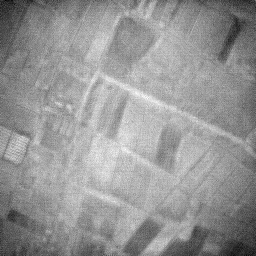
\includegraphics[width=6.4cm,height=6.4cm]{../filt_fake.png}};
\coordinate (out1-east) at (output-anchor);

\draw [connection]  (cnr_b6-east)    -- node {\midarrow}  (output-west);

\pic[shift={(-8,-12,0)}] at (bottleneck.north) 
    {Box={
        name=convS1_legend,
        caption={$7 \times 7 \; \text{Conv}$ $\text{Stride}=1$},
        xlabel={{, }},
        zlabel=,
        fill = \StrideOneColor,
        height=6,
        width=1,
        depth=6,
        xlabeloc=0.5,
        }
    };

\pic[shift={(4,0,0)}] at (convS1_legend-east) 
    {Box={
        name=convS2_legend,
        caption={$3 \times 3 \; \text{Conv}$ $\text{Stride}=2$},
        xlabel={{, }},
        zlabel=,
        fill = \StrideTwoColor,
        height=6,
        width=1,
        depth=6,
        xlabeloc=0.5,
        }
    };

\pic[shift={(4,0,0)}] at (convS2_legend-east) 
    {Box={
        name=res_block_legend,
        caption=Residual Block,
        xlabel={{, }},
        zlabel=,
        fill = \ResBlocksColor,
        height=6,
        width=1,
        depth=6,
        xlabeloc=0.5,
        }
    };

\pic[shift={(4,0,0)}] at (res_block_legend-east) 
    {Box={
        name=trans_conv_legend,
        caption={$3 \times 3 \; \text{Trans.}$ $\text{Conv}$},
        xlabel={{, }},
        zlabel=,
        fill = \TransConvColor,
        height=6,
        width=1,
        depth=6,
        xlabeloc=0.5,
        }
    };

\pic[shift={ (4,0,0) }] at (trans_conv_legend-east) 
    {RightBandedBox={
        name=res_block_legend,
        caption=InstanceNorm + ReLU,
        xlabel={{, }},
        zlabel=,
        fill=\ConvColor,
        bandfill=\ConvReluColor,
        height=6,
        width=1,
        depth=6,
        opacity = 0.6,
        bandopacity = 0.6
        }
    };

\end{tikzpicture}
\end{document}
